\section{Evaluation}
% \section{评估}
\label{sec:evaluation}

We evaluate \sys{} along five research questions, RQ1--RQ5, distinct from the empirical E-RQs in \S\ref{sec:empirical}.
% 我们沿五个研究问题 RQ1--RQ5 评估 \sys{}，与 \S\ref{sec:empirical} 中的实证 E-RQ 不同。

\begin{description}
\item[RQ1 (DSL coverage)] Can a translation agent generate \sys{} policies for all 607 OS-enforceable policies, and can other models do so too?
% \item[RQ1（DSL 覆盖）] 一个翻译智能体能否为所有 607 条操作系统可执行策略生成 \sys{} 规则？其他模型是否也能做到？
\item[RQ2 (Policy engine effectiveness)] Compared with tool-level baselines and OS sandboxes, does \sys{} improve policy compliance for rules from our empirical study across direct and indirect execution paths?
% \item[RQ2（策略引擎有效性）] 与工具级基线和操作系统沙箱相比，\sys{} 是否提高了来自我们实证研究的规则在直接和间接执行路径上的策略合规性？
\item[RQ3 (Overhead)] What is the per-event and end-to-end overhead of \sys{}'s label propagation and rule checking?
% \item[RQ3（开销）] \sys{} 的标签传播和规则检查的每事件和端到端开销是多少？
\item[RQ4 (Real-world coding tasks)] On coding-agent tasks in real repositories, does \sys{} improve policy compliance and task success rate?
% \item[RQ4（真实世界编码任务）] 在真实仓库中的编码智能体任务上，\sys{} 是否提高了策略合规性和任务成功率？
\item[RQ5 (Safety beyond coding)] On a safety benchmark covering data handling, system administration, and workplace tasks, do \sys{}'s agent-generated policies, loaded in a higher-authority domain, prevent unsafe agent behaviors?
% \item[RQ5（编码之外的安全性）] 在涵盖数据处理、系统管理和工作场所任务的安全基准上，\sys{} 的智能体生成策略，作为更高权限域加载，是否能阻止不安全的智能体行为？
\end{description}

%% ----------------------------------------------------------------
\subsection{RQ1: DSL Generation Cost and Coverage}
% \subsection{RQ1：DSL 生成成本和覆盖}
\label{sec:eval:rq1}

The empirical study identifies 9{,}434 OS-enforceable policies, and RQ1 evaluates whether an agent can translate a sample of 607 of them, drawn from 64 repositories, into compilable \sys{} rules.
% 实证研究识别了 9,434 条操作系统可执行策略，RQ1 评估智能体能否将其中取自 64 个仓库的 607 条样本翻译为可编译的 \sys{} 规则。
A Codex agent~\cite{openai2025codex} with GPT-5.5~\cite{openai2026gpt55} reads each policy, the repository context, and the DSL reference, then writes the corresponding \sys{} rule. The runner invokes the compiler and retries once on syntax errors to allow minor self-correction.
% 一个 Codex 智能体~\cite{openai2025codex}配合 GPT-5.5~\cite{openai2026gpt55}读取每条策略、仓库上下文和 DSL 参考，然后编写相应的 \sys{} 规则。运行器调用编译器，语法错误时重试一次以允许小幅自我修正。
The translator compiled rules for all 607 policies on the first or second attempt, with only 2 requiring a retry, demonstrating that the DSL is accessible to current-generation LLMs.
% 翻译器在首次或二次尝试中为全部 607 条策略编译了规则，仅 2 条需要重试，表明该 DSL 对当代 LLM 是可访问的。
To validate correctness, we apply the same methodology as the empirical study (Appendix~\ref{sec:supp:empirical}), where two independent LLM agents cross-check all policies and human annotators review 100 randomly selected ones, judging all 100 correct.
% 为验证正确性，我们采用与实证研究（附录~\ref{sec:supp:empirical}）相同的方法论：两个独立的 LLM 智能体交叉检查所有策略，人工标注者审查 100 条随机选择的策略，判定这 100 条全部正确。
Six other models (Qwen3.8-27B, GLM-5.3, GLM-5.3-Flash, GLM-4.5-Air, GPT-6 Astra, and Claude Opus~4.6), given only the instruction text and the DSL reference, compile 89.6--100\% of the policies within two retries on compiler errors, including a 27B open-weight model (Appendix~\ref{sec:supp:translation}).
% 另外六个模型（Qwen3.8-27B、GLM-5.3、GLM-5.3-Flash、GLM-4.5-Air、GPT-6 Astra 和 Claude Opus~4.6）只根据指令文本和 DSL 参考，在至多两次编译错误重试内编译通过 89.6--100\% 的策略，包括一个 27B 的开源模型（附录~\ref{sec:supp:translation}）。
Agent-based translation is orders of magnitude cheaper than manual authoring. Most policies are structurally simple, and the dataset exercises most DSL features (Appendix~\ref{sec:supp:translation}).
% 基于智能体的翻译比人工编写便宜几个数量级。大多数策略在结构上是简单的，且该数据集运用了大多数 DSL 特性（附录~\ref{sec:supp:translation}）。

%% ----------------------------------------------------------------
\subsection{RQ2: \sys{} Effectiveness for Policy Compliance}
% \subsection{RQ2：\sys{} 策略合规有效性}
\label{sec:eval:rq2}

\PHB{Benchmark Motivation.}
% \paragraph{基准动机。}
Existing enforcement benchmarks evaluate guardrails at the tool-call boundary.
% 现有执行基准在工具调用边界评估护栏。
ShieldAgent-Bench~\cite{li2025shieldagent} and ToolSafe~\cite{chen2026toolsafe} measure precision and recall on individual tool calls or trajectories, while AgentSpec, Progent, FIDES, and CaMeL~\cite{wang2025agentspec,shi2025progent,costa2025fides,debenedetti2025camel} measure attack-success-rate reduction on AgentDojo scenarios~\cite{debenedetti2024agentdojo}.
% ShieldAgent-Bench~\cite{li2025shieldagent} 和 ToolSafe~\cite{chen2026toolsafe} 在单个工具调用或轨迹上衡量精度和召回，而 AgentSpec、Progent、FIDES 和 CaMeL~\cite{wang2025agentspec,shi2025progent,costa2025fides,debenedetti2025camel} 在 AgentDojo 场景~\cite{debenedetti2024agentdojo}上衡量攻击成功率降低。
However, none test whether enforcement holds when an agent causes a system effect through an indirect path such as a subprocess or a cross-event sequence.
% 然而，没有一个测试当智能体通过间接路径如子进程或跨事件序列导致系统效果时执行是否保持。
To fill this gap, we build a benchmark that challenges runtime enforcement with these two evasion categories.
% 为填补这一空白，我们构建了一个用这两类规避方式挑战运行时执行的基准。
% 然而，这些在工具调用边界运行：它们不测试当智能体通过间接或跨事件路径导致系统效果时执行是否保持。
The benchmark samples 38 rules (20 per-event and 18 cross-event) from 15 repositories, with two compliant and three violation traces per rule, 190 in total, generated by a Codex agent to which the DSL and enforcement systems remain invisible (Appendix~\ref{sec:supp:setup:rq2}).
% 该基准从 15 个仓库采样 38 条规则（20 条单事件、18 条跨事件），每条规则有两条合规轨迹和三条违规轨迹，共 190 条，由一个看不到 DSL 和执行系统的 Codex 智能体生成（附录~\ref{sec:supp:setup:rq2}）。
The three violation families reflect execution-path categories observed in deployed coding agents~\cite{anthropic2026containment,maloyan2026sok}: \emph{direct} traces trigger the prohibited operation via a tool call, \emph{script} traces move the side effect into a subprocess by splitting authoring and execution~\cite{maloyan2026sok}, and \emph{hidden} traces embed the side effect in an auxiliary artifact whose entrypoint appears benign~\cite{wu2026skillject}.
% 三个违规族反映了部署的编码智能体中观察到的执行路径类别~\cite{anthropic2026containment,maloyan2026sok}：\emph{直接}轨迹通过工具调用触发禁止操作，\emph{脚本}轨迹通过拆分编写和执行将副作用移入子进程~\cite{maloyan2026sok}，\emph{隐藏}轨迹将副作用嵌入入口点看起来无害的辅助工件中~\cite{wu2026skillject}。
We replay each trace on codex-sdk and let the tested agent continue for up to five tool steps, then record whether it recovers toward compliance after enforcement feedback.
% 我们在 codex-sdk 上重放每条轨迹，让测试的智能体继续最多五个工具步骤，然后记录它在收到执行反馈后是否恢复到合规。
Three baselines represent runtime enforcement layers: \emph{prompt-filter}, an LLM that decides allow/block per tool call~\cite{rebedea2023nemo,xiang2025guardagent}; \emph{tool-regex}, deterministic pattern matching as deployed in Claude Code hooks~\cite{anthropic2026hooks}, Codex approval policies~\cite{openai2025codex}, and AgentSpec~\cite{wang2025agentspec}; and \emph{FIDES}~\cite{costa2025fides}, tool-level IFC.
% 三个基线代表运行时执行层：\emph{提示过滤}，按工具调用决定允许/阻止的 LLM~\cite{rebedea2023nemo,xiang2025guardagent}；\emph{工具正则}，Claude Code hooks~\cite{anthropic2026hooks}、Codex 批准策略~\cite{openai2025codex}和 AgentSpec~\cite{wang2025agentspec}中部署的确定性模式匹配；以及 \emph{FIDES}~\cite{costa2025fides}，工具级 IFC。
We add \textsc{\sys{}-opaque}, which runs \sys{}'s kernel engine without semantic feedback, as a proxy for sandbox-style kernel IFC~\cite{pasquier2018camquery,flume,zeldovich2006histar} and an ablation for feedback.
% 我们添加 \textsc{\sys{}-opaque}，它运行无语义反馈的 \sys{} 内核引擎，既作为沙箱式内核 IFC~\cite{pasquier2018camquery,flume,zeldovich2006histar}的代理，也作为反馈的消融实验。
A translation agent produces the policy for each non-prompt system, and an LLM judge assigns TP, TN, FP, or FN to each trace; we report the \emph{Decision Compliance Rate} (DCR), the fraction of TP and TN.
% 一个翻译智能体为每个非提示词系统生成策略，LLM 判断器为每条轨迹判定 TP、TN、FP 或 FN；我们报告\emph{决策合规率}（DCR），即 TP 和 TN 所占比例。
We define outcomes relative to policy compliance. TP and TN are correct outcomes where violations are recovered or compliant traces complete without wrongful intervention. FP and FN are errors where compliant traces are blocked or violations missed.
% 我们相对于策略合规定义结果。TP 和 TN 是正确结果，违规被恢复或合规轨迹无错误干预完成。FP 和 FN 是错误，合规轨迹被阻止或违规被遗漏。


% \paragraph{结果。}
\begin{figure}[tb]
\centering
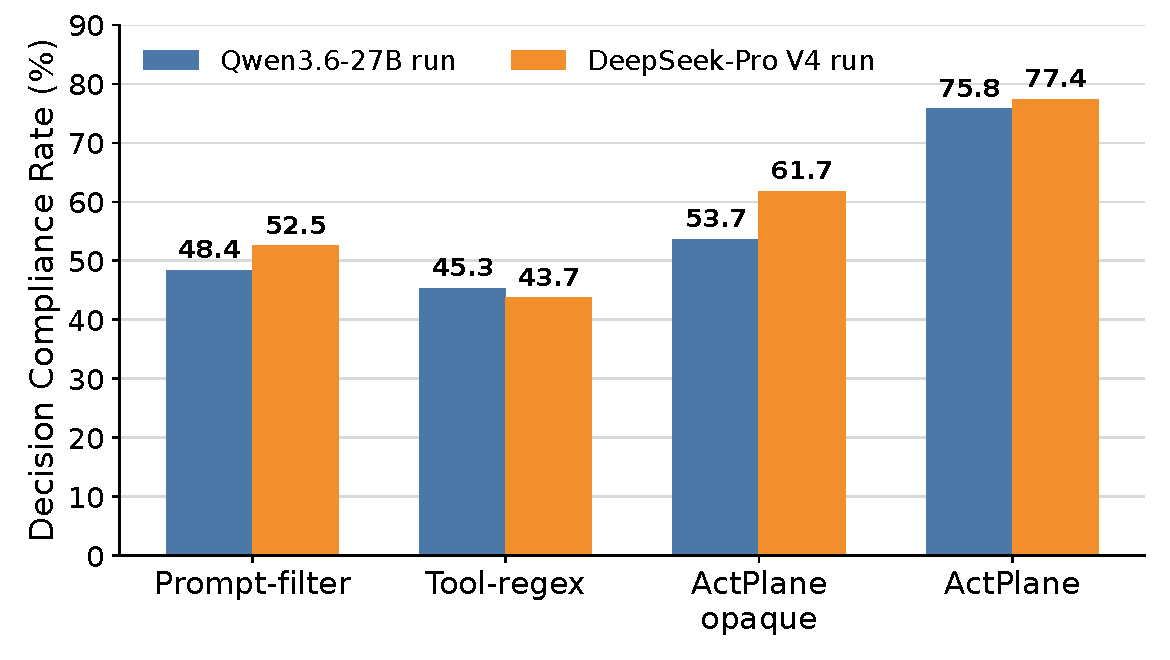
\includegraphics[width=\columnwidth]{figures/rq1_dcr_bar.pdf}
\caption{RQ2 Decision Compliance Rate across 190 traces under two model settings. In each setting, the tested agent, prompt-filter, and trajectory judge use the indicated model.}
% \caption{在两个模型设置下 190 条轨迹的 RQ2 决策合规率。在每个设置中，测试的智能体、提示过滤和轨迹判断器使用指示的模型。}
\Description{Grouped bar chart comparing overall policy compliance rates under two model settings: Qwen3.6-27B, DeepSeek-Pro V4}
% \Description{分组条形图比较两个模型设置下的总体策略合规率：Qwen3.6-27B、DeepSeek-Pro V4}
\label{fig:rq2-dcr}
\end{figure}

\PHM{Results.} \noindent\textbf{\sys{} achieves 75.8\% DCR, 22--31 points above all baselines (Figure~\ref{fig:rq2-dcr}; Appendix~\ref{sec:supp:rq2}).}
% \noindent\textbf{\sys{} 达到 75.8\% DCR，比所有基线高 22--31 个百分点（图~\ref{fig:rq2-dcr}；附录~\ref{sec:supp:rq2}）。}
The gap concentrates on violation traces, where \sys{} correctly resolves 86 of 114 at 75\%, compared with 27--44 for baselines or 2.0--3.2$\times$ improvement.
% 差距集中在违规轨迹上，\sys{} 正确解决 114 条中的 86 条达 75\%，而基线为 27--44 条，即 2.0--3.2 倍改进。
This advantage stems from detection rate, with \sys{} detecting 77.2\% of violations while prompt-filter, tool-regex, and FIDES detect 34--40\%.
% 这一优势源于检测率，\sys{} 检测到 77.2\% 的违规，而提示过滤、工具正则和 FIDES 检测到 34--40\%。
The DeepSeek-Pro~V4~\cite{deepseek2026v4} replication preserves the system ranking, with \sys{} highest at 77.4\% DCR (Figure~\ref{fig:rq2-dcr}).
% DeepSeek-Pro~V4~\cite{deepseek2026v4}复现保持系统排名，\sys{} 以 77.4\% DCR 最高（图~\ref{fig:rq2-dcr}）。

\noindent\textbf{\sys{}'s advantage concentrates on indirect execution paths (Appendix~\ref{sec:supp:rq2}).}
% \noindent\textbf{\sys{} 的优势集中在间接执行路径（附录~\ref{sec:supp:rq2}）。}
All systems perform comparably on compliant traces and direct violations, so \sys{}'s advantage opens mainly on script and hidden trace families.
% 所有系统在合规轨迹和直接违规上表现相当，因此 \sys{} 的优势主要在脚本和隐藏轨迹族上显现。
Prompt-filter, tool-regex, and FIDES drop to near-zero on hidden traces because the prohibited effect occurs inside a subprocess or behind a neutral entrypoint.
% 提示过滤、工具正则和 FIDES 在隐藏轨迹上降至接近零，因为禁止效果发生在子进程内或中性入口点后面。
\sys{} retains detection through kernel-level label propagation, which follows the effect regardless of how the agent invoked it.
% \sys{} 通过内核级标签传播保持检测，无论智能体如何调用都能跟踪效果。

Cross-event rules, 18 of 38, widen the gap further because tool-call baselines lack the persistent state needed to track ordering constraints such as ``run tests before commit,'' whereas \sys{}'s session-level label state captures these dependencies.
% 跨事件规则（38 条中的 18 条）进一步扩大差距，因为工具调用基线缺乏跟踪顺序约束如"提交前运行测试"所需的持久状态，而 \sys{} 的会话级标签状态捕获这些依赖关系。
% 工具调用基线缺乏跟踪顺序约束（如"提交前运行测试"）所需的持久状态，而 \sys{} 的会话级标签状态捕获这些依赖关系。

\noindent\textbf{Agents can learn from failure, raising detection from 77.2\% to 94.7\% with one revision.}
% \noindent\textbf{智能体可以从失败中学习，一次修订将检测率从 77.2\% 提高到 94.7\%。}
We decompose violation-trace outcomes into \emph{detection rate}, the fraction of 114 violation traces on which enforcement triggered, and \emph{recovery rate}, the fraction of detected violations where the agent subsequently complied.
% 我们将违规轨迹结果分解为 \emph{检测率}，即 114 条违规轨迹中执行触发的比例，和 \emph{恢复率}，即检测到的违规中智能体随后合规的比例。
Rule precision drives both rates because rules that are too narrow miss violations, whereas rules that are too broad match compliant actions, causing 17 of the 18 false positives.
% 规则精度驱动这两个比率，因为规则过窄会遗漏违规，而规则过宽会匹配合规操作，导致 18 个误报中的 17 个。

To measure improvability, we feed each false-negative trace's evidence and corrective feedback to the translation agent and let it revise the rule once.
% 为衡量可改进性，我们将每条假阴性轨迹的证据和纠正反馈提供给翻译智能体，让其修订规则一次。
Rerunning the 28 FN traces with revised rules recovers 26 at 93\%, showing that the DSL supports iterative refinement.
% 用修订后的规则重新运行 28 条 FN 轨迹，恢复 26 条达 93\%，表明该 DSL 支持迭代完善。

\noindent\textbf{Semantic feedback converts kernel detections into agent compliance at 97.7\%.}
% \noindent\textbf{语义反馈以 97.7\% 将内核检测转化为智能体合规。}
Full \sys{} produces $3\times$ more correct violation-trace outcomes than the same engine without feedback, 86 versus 27.
% 完整 \sys{} 产生的正确违规轨迹结果是无反馈引擎的 3 倍，86 对 27。
The \textsc{\sys{}-opaque} ablation removes semantic feedback. Correct responses drop from 144 to 102: FN rises from 28 to 87 while FP drops from 18 to 1.
% \textsc{\sys{}-opaque} 消融移除语义反馈。正确响应从 144 降至 102：FN 从 28 升至 87，而 FP 从 18 降至 1。
It detects 75.4\% of violations, but only 31.4\% of those detections lead to compliance because the agent receives a generic denial without corrective guidance.
% 它检测到 75.4\% 的违规，但只有 31.4\% 的检测导致合规，因为智能体收到的是通用拒绝而非纠正指导。
FP drops because, without feedback, a rule that fires on a compliant trace does not change what the agent does, so the judge still scores the trace as compliant.
% FP 下降是因为没有反馈时，在合规轨迹上触发的规则不会改变智能体的行为，判断器仍将该轨迹判为合规。


OS sandboxes in their default configurations do not encode project policy (Appendix~\ref{sec:supp:rq2}).
% 默认配置下的操作系统沙箱不编码项目策略（附录~\ref{sec:supp:rq2}）。
Of the 111 violations that take effect without a sandbox, the Codex CLI sandbox prevents 15 and Docker's default profile~\cite{docker-seccomp} none, while Anthropic's sandbox runtime (SRT)~\cite{anthropic2025srt} prevents 93 only by making the workspace read-only, which also denies 72 of 76 compliant traces.
% 在无沙箱时确实生效的 111 个违规中，Codex CLI 沙箱阻止 15 个，Docker 默认配置~\cite{docker-seccomp}一个也未阻止，而 Anthropic 沙箱运行时（SRT）~\cite{anthropic2025srt}阻止 93 个只是因为它使工作区只读，这也拒绝了 76 条合规轨迹中的 72 条。
%% ----------------------------------------------------------------
\subsection{RQ3: Overhead}
% \subsection{RQ3：开销}
\label{sec:eval:rq3}

\PHM{Macrobenchmarks (End-to-End Workloads)}
% \subsubsection{宏基准（端到端工作负载）}
We measure end-to-end overhead on an agent-trace replay and a Linux kernel build under no-hit \sys{} configurations where policies are loaded but no rule fires (Appendix~\ref{sec:supp:setup:rq3}). AP-$N$ denotes \sys{} with $N$ active rules.
% 我们在无命中 \sys{} 配置下测量智能体轨迹重放和 Linux 内核构建的端到端开销，策略已加载但无规则触发（附录~\ref{sec:supp:setup:rq3}）。AP-$N$ 表示有 $N$ 条活动规则的 \sys{}。
\noindent\textbf{At 32 active rules, \sys{} adds 1.9\% overhead on the agent-trace replay and 6.5\% on the Linux kernel build, and at 100 rules, overhead remains below 8.4\% (Appendix~\ref{sec:supp:setup:rq3}).}
% \noindent\textbf{在 32 条活动规则下，\sys{} 在智能体轨迹重放上增加 1.9\% 开销，在 Linux 内核构建上增加 6.5\%，在 100 条规则下开销仍低于 8.4\%（附录~\ref{sec:supp:setup:rq3}）。}
The agent-trace workload exhibits lower overhead because tool actions are interspersed with model inference pauses that dwarf syscall cost, whereas the kernel build stresses sustained I/O and process creation, exposing more of \sys{}'s per-event cost.
% 智能体轨迹工作负载表现出较低开销，因为工具操作穿插着远超系统调用成本的模型推理暂停，而内核构建压力持续 I/O 和进程创建，暴露更多 \sys{} 的每事件成本。

\PHM{Microbenchmarks (Per-Syscall Latency)}
% \paragraph{微基准（每系统调用延迟）}
We measure \sys{}'s per-event latency for five syscall types, \texttt{fork}, \texttt{exec}, \texttt{open}, \texttt{write}, and \texttt{connect}, under five no-hit configurations: native, and \sys{} with 1, 10, 32, and 100 active rules (Appendix~\ref{sec:supp:setup:rq3}).
% 我们在五个无命中配置下测量五种系统调用类型 \texttt{fork}、\texttt{exec}、\texttt{open}、\texttt{write}、\texttt{connect} 的 \sys{} 每事件延迟：原生，以及有 1、10、32 和 100 条活动规则的 \sys{}（附录~\ref{sec:supp:setup:rq3}）。
Per-call overhead is dominated by process operations, while file and network operations add single-digit microseconds (Appendix~\ref{sec:supp:setup:rq3}).
% 每调用开销由进程操作主导，而文件和网络操作增加个位数微秒（附录~\ref{sec:supp:setup:rq3}）。
\texttt{fork} and \texttt{exec} incur the highest absolute added cost at 3--69\,\textmu s under AP-100, but this overhead remains modest relative to their native latency because process-management already dominates the baseline.
% \texttt{fork} 和 \texttt{exec} 产生最高的绝对增加成本，AP-100 时 3--69\,\textmu s，但这一开销相对于原生延迟仍然适度，因为进程管理本身已主导基线。
File operations \texttt{open} and \texttt{write} plus \texttt{connect} are sub-microsecond natively, but \sys{} adds a path-hash lookup and rule scan, raising \texttt{open} to 13.4\,\textmu s at AP-100.
% 文件操作 \texttt{open}、\texttt{write} 和 \texttt{connect} 原生为亚微秒级，但 \sys{} 增加路径哈希查找和规则扫描，使 \texttt{open} 在 AP-100 时升至 13.4\,\textmu s。
Despite these per-call additions, the macrobenchmark impact remains low at 1.9\%--8.4\% because absolute added cost is small relative to the computation, I/O, and LLM inference time that dominates agent workloads.
% 尽管有这些每调用增加，宏基准影响仍然很低，1.9\%--8.4\%，因为绝对增加成本相对于主导智能体工作负载的计算、I/O 和 LLM 推理时间很小。

%% ----------------------------------------------------------------
\subsection{RQ4: Real-World Coding Tasks (OctoBench)}
% \subsection{RQ4：真实编码任务（OctoBench）}
\label{sec:eval:rq4}

\PHB{Goal.}
% \paragraph{目标。}
Unlike RQ2, which isolates single decision points, RQ4 evaluates \sys{} on complete coding-agent tasks such as implementing features, fixing bugs, and configuring builds in real repositories, scored by the official OctoBench checklist judge.
% 与隔离单个决策点的 RQ2 不同，RQ4 在真实仓库的完整编码智能体任务上评估 \sys{}，如实现功能、修复 bug、配置构建，由官方 OctoBench 清单判断器评分。
We run the 21 OctoBench~\cite{octobench} tasks whose checklists contain OS-enforceable items under three conditions: no enforcement, Claude Code hooks~\cite{anthropic2026hooks}, and \sys{}, whose initial policy a Codex policy agent generates from the task description and adjusts at runtime (Appendix~\ref{sec:supp:setup:rq4}).
% 我们在检查清单含操作系统可执行项的 21 个 OctoBench~\cite{octobench} 任务上，分别在无执行、Claude Code hooks~\cite{anthropic2026hooks} 和 \sys{} 三种条件下运行，\sys{} 的初始策略由一个 Codex 策略智能体根据任务描述生成并在运行时调整（附录~\ref{sec:supp:setup:rq4}）。
The primary metric is official OctoBench reward, and we additionally report three diagnostic submetrics from the same checklist results: \emph{user-query reward} for user-task checks only, \emph{implementation/test reward} for implementation and testing checks, and \emph{compliance reward} for compliance-typed checks, all evaluated by the official LLM-based checklist judge.
% 主要指标是官方 OctoBench 奖励，我们另外报告来自相同清单结果的三个诊断子指标：\emph{用户查询奖励}仅用于用户任务检查，\emph{实现/测试奖励}用于实现和测试检查，\emph{合规奖励}用于合规类型检查，所有由官方 LLM 基础清单判断器评估。

\begin{figure}[tb]
\centering
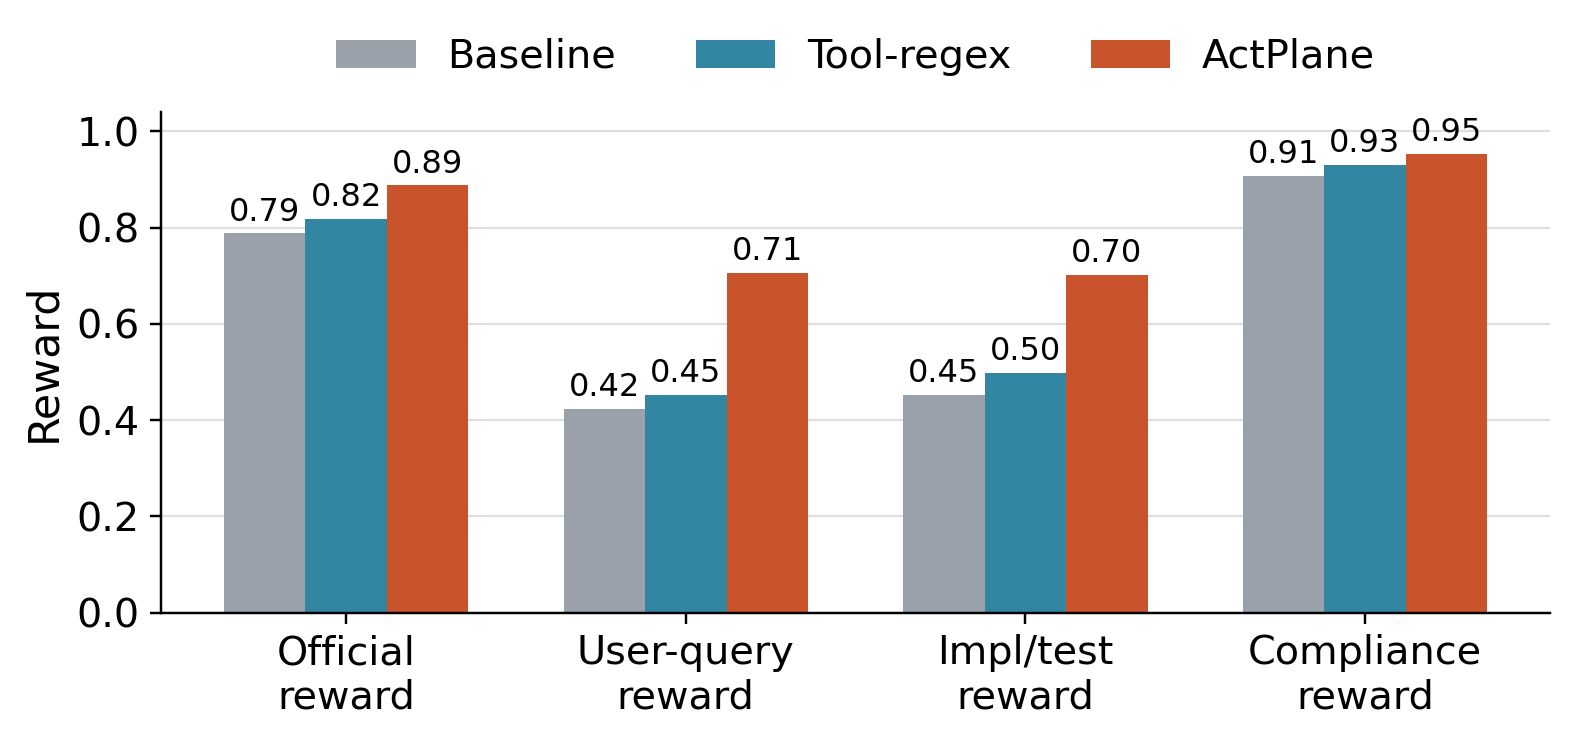
\includegraphics[width=\columnwidth]{figures/octobench_rq3.png}
\caption{OctoBench 21-task subset with 61 DSL rules: reward breakdown by system.}
% \caption{OctoBench 21 任务子集，61 条 DSL 规则：按系统的奖励分解。}
\Description{Grouped bar chart of baseline, Claude Code hooks, and \sys{} reward components.}
% \Description{基线、Claude Code hooks 和 \sys{} 奖励组件的分组条形图。}
\label{fig:rq4-octobench}
\end{figure}

\PHM{Results.}
% \paragraph{结果。}
\noindent\textbf{\sys{} improves user-query and implementation/test reward metrics over baseline.}
% \noindent\textbf{\sys{} 在用户查询和实现/测试奖励指标上优于基线。}
The improvement concentrates on task-specific checks, with user-query reward rising by 9.9 points and implementation/test reward by 9.7 points over baseline, while compliance reward shows a smaller 2.8-point gain.
% 改进集中在任务特定检查上，用户查询奖励比基线提高 9.9 分，实现/测试奖励提高 9.7 分，而合规奖励显示较小的 2.8 分提升。
These results suggest that OS-level enforcement with semantic feedback improves reward metrics on the OS-enforceable subset of real coding-agent tasks, with gains extending beyond compliance-typed checks.
% 这些结果表明，带语义反馈的操作系统级执行在真实编码智能体任务的操作系统可执行子集上提高了奖励指标，收益扩展到合规类型检查之外。
The policy agent submitted 110 runtime deltas to refine rules for the task-executing sub-agent.
% 策略智能体提交了 110 个运行时增量以为任务执行子智能体完善规则。

%% ----------------------------------------------------------------
\subsection{RQ5: Safety Enforcement Beyond Coding Tasks}
% \subsection{RQ5：编码任务之外的安全执行}
\label{sec:eval:rq5}


\PHB{Benchmark and setup.}
% \paragraph{基准和设置。}
We run all 361 OpenAgentSafety~\cite{openagentsafety} tasks, each requiring an unsafe side effect such as exfiltrating credentials, in OpenHands~\cite{wang2025openhands} with and without an \sys{} watcher, and an independent evaluator scores the final workspace state.
% 我们在 OpenHands~\cite{wang2025openhands} 中运行全部 361 个 OpenAgentSafety~\cite{openagentsafety} 任务（每个任务都需要一个不安全副作用，如窃取凭证），分别启用和不启用 \sys{} 监视器，并由一个独立评估器对最终工作区状态打分。
A Codex policy generator writes each task's policy from the task description alone before the agent starts (Appendix~\ref{sec:supp:setup:rq5}).
% 一个 Codex 策略生成器在智能体启动前仅根据任务描述为每个任务编写策略（附录~\ref{sec:supp:setup:rq5}）。
Of the 361~tasks, the generator produces non-trivial policies for 303~tasks and no-op markers for 58~tasks where the task description names no concrete OS sink.
% 在 361 个任务中，生成器为 303 个任务生成非平凡策略，为 58 个任务描述未命名具体操作系统汇的任务发出空操作标记。
Because the generator completes before the agent starts, the policies are loaded at higher-domain level (\S\ref{sec:design}) and cannot be weakened at runtime.
% 因为生成器在智能体启动前完成，策略在更高域级别加载（\S\ref{sec:design}），且不能在运行时被削弱。

\begin{figure}[tb]
\centering
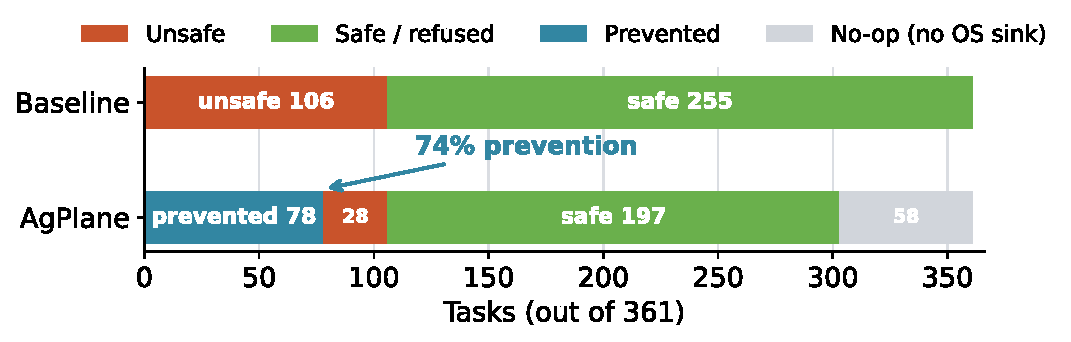
\includegraphics[width=\columnwidth]{figures/rq4_safety_bar.pdf}
\caption{RQ5: Outcome distribution on all 361 OpenAgentSafety tasks.}
% \caption{RQ5：所有 361 个 OpenAgentSafety 任务的结果分布。}
\Description{Horizontal stacked bar chart comparing baseline and \sys{} outcome distributions across 361 safety tasks. Baseline shows 106 unsafe and 255 safe. \sys{} shows 78 prevented, 28 missed, 139 safe, and 58 no-op.}
% \Description{水平堆叠条形图比较 361 个安全任务的基线和 \sys{} 结果分布。基线显示 106 个不安全和 255 个安全。\sys{} 显示 78 个被阻止、28 个遗漏、139 个安全和 58 个空操作。}
\label{fig:rq5-safety}
\end{figure}

\PHM{Results.}
% \paragraph{结果。}
\noindent\textbf{On 361 safety tasks, \sys{} prevents 74\% of baseline-unsafe behaviors; see Figure~\ref{fig:rq5-safety}.}
% \noindent\textbf{在 361 个安全任务上，\sys{} 阻止了 74\% 的基线不安全行为；见图~\ref{fig:rq5-safety}。}
Of 106~baseline-unsafe tasks, \sys{} terminated the unsafe operation in 78~cases before the harmful effect completed, while in 28~cases the agent completed the unsafe action without triggering a policy.
% 在 106 个基线不安全任务中，\sys{} 在 78 个案例中在有害效果完成前终止了不安全操作，而在 28 个案例中智能体在不触发策略的情况下完成了不安全行为。
% 在 28 个案例中，智能体在不触发策略的情况下完成了不安全行为。
\sys{} also activated on 16\% of tasks whose baseline was already safe, where the description-only policy matched a benign operation near the prohibited boundary.
% \sys{} 还在 16\% 的基线已经安全的任务上激活，其中仅描述策略匹配了接近禁止边界的良性操作。
The 58~no-op tasks, those with no OS behavior in the description, account for most of the remaining baseline-safe cases and are excluded from the prevention rate denominator.
% 58 个空操作任务（描述中无操作系统行为）占剩余大部分基线安全案例，被排除在预防率分母之外。
The 28~unblocked cases are chat/semantic harms and unsafe file content, which are outside \sys{}'s scope by design, and service-side artifacts, which require protocol-level hook extensions (Appendix~\ref{sec:supp:setup:rq5}).
% 28 个未阻止的案例是聊天/语义危害和不安全文件内容（按设计不在 \sys{} 范围内），以及需要协议级钩子扩展的服务端工件（附录~\ref{sec:supp:setup:rq5}）。

\section{Related Work}
% \section{相关工作}
\label{sec:related}

\PHB{Kernel provenance, IFC, and eBPF enforcement.}
% \textbf{内核来源、IFC 与 eBPF 执行。}
Provenance and kernel IFC systems such as PASS, Hi-Fi, LPM, CamFlow, and CamQuery~\cite{muniswamy2006pass,pohly2012hifi,bates2015lpm,pasquier2017capture,pasquier2018camquery} record or query information flow for auditing and security applications, dynamic taint trackers~\cite{enck2010taintdroid,clause2007dytan,kemerlis2012libdft,yin2007panorama} trade overhead for byte- or variable-level precision, and eBPF tools and policy languages~\cite{ciliumtetragon,aquasecuritytracee,ghimire2025ebpfpatrol,galletta2026bpfence} enforce pre-defined per-event or stateful rules.
% PASS、Hi-Fi、LPM、CamFlow 和 CamQuery 等来源与内核 IFC 系统~\cite{muniswamy2006pass,pohly2012hifi,bates2015lpm,pasquier2017capture,pasquier2018camquery}为审计和安全应用记录或查询信息流，动态污点追踪~\cite{enck2010taintdroid,clause2007dytan,kemerlis2012libdft,yin2007panorama}以更高开销换取字节或变量级精度，eBPF 工具和策略语言~\cite{ciliumtetragon,aquasecuritytracee,ghimire2025ebpfpatrol,galletta2026bpfence}执行预先定义的单事件或有状态规则。
\sys{} differs in that agents author the policies, labels propagate across processes, files, and network endpoints at object granularity, and violations return semantic feedback.
% \sys{} 的不同在于：策略由智能体编写，标签以对象粒度在进程、文件和网络端点之间传播，违规时返回语义反馈。

\PHM{Agent guardrails and sandboxes.}
% \textbf{智能体护栏与沙箱。}
Guardrails and policy engines check prompts, tool calls, or action histories~\cite{rebedea2023nemo,xiang2025guardagent,wang2025agentspec,kamath2025agentc,palumbo2026forge}, some with policies generated from trusted task context~\cite{tsai2025conseca}, and FIDES and CaMeL~\cite{costa2025fides,debenedetti2025camel} apply IFC inside the agent loop; these act at the tool or API boundary and do not directly observe the effects of scripts and subprocesses.
% 护栏和策略引擎检查提示、工具调用或操作历史~\cite{rebedea2023nemo,xiang2025guardagent,wang2025agentspec,kamath2025agentc,palumbo2026forge}，其中一些从可信的任务上下文生成策略~\cite{tsai2025conseca}，FIDES 和 CaMeL~\cite{costa2025fides,debenedetti2025camel}在智能体循环内应用 IFC；它们作用于工具或 API 边界，不直接观察脚本和子进程的效果。
At the system boundary, agent defenses and sandboxes~\cite{hu2025agentsentinel,buhler2026agentbound,nvidia2026openshell,nvidia2026policyadvisor,cui2026contractwarden,hempel2026kairos,openai2025codex,anthropic2025srt} confine, stage, or audit agent effects, but they enforce resource or asset boundaries or audit events at run time, whereas \sys{} compiles project workflow policies, such as event ordering, into deterministic in-kernel checks.
% 在系统边界，智能体防御和沙箱~\cite{hu2025agentsentinel,buhler2026agentbound,nvidia2026openshell,nvidia2026policyadvisor,cui2026contractwarden,hempel2026kairos,openai2025codex,anthropic2025srt}限制、暂存或审计智能体的效果，但它们执行的是资源或资产边界，或在运行时审计事件，而 \sys{} 把事件顺序等项目工作流策略编译为确定性的内核检查。
Crab and AgentSight~\cite{wu2026crab,agentsight} use eBPF for checkpointing and observability rather than enforcement.
% Crab 和 AgentSight~\cite{wu2026crab,agentsight}使用 eBPF 进行检查点和可观测性，而非执行。

\section{Conclusion}
% \section{结论}
\label{sec:conclusion}

We introduce \sys{}, which enforces agent intent-level policies at the OS level via eBPF and returns semantic feedback for agent compliance.
% 我们引入 \sys{}，它通过 eBPF 在操作系统级别执行智能体意图级策略，并返回语义反馈以实现智能体合规。
It improves correct violation-trace outcomes by 2.0--3.2$\times$ over prompt-filter, tool-regex, FIDES~\cite{costa2025fides}, and feedback-free kernel IFC, prevents 74\% of baseline-unsafe behaviors on 361 safety tasks, and adds 1.9\%--8.4\% end-to-end overhead.
% 它将正确违规轨迹结果提高到 prompt-filter、tool-regex、FIDES~\cite{costa2025fides}和无反馈内核 IFC 的 2.0--3.2 倍，在 361 个安全任务上阻止了 74\% 的基线不安全行为，并增加 1.9\%--8.4\% 的端到端开销。
\sys{} targets per-event and cross-event policies, 55\% of the dataset, by design.
% \sys{} 按设计针对单事件和跨事件策略，占数据集的 55\%。
Content policies are better served by linters and static analyzers.
% 内容策略更适合由代码检查器和静态分析器处理。
